\begin{tikzpicture}[x=1cm,y=1cm,>=Stealth,font=\small,
  req/.style={draw=blue!35!black,fill=blue!66!gray,text=white,rounded corners=2pt,
    minimum width=2.15cm,minimum height=.65cm,align=center},
  ability/.style={draw=blue!35!black,fill=green!40!black,text=white,rounded corners=2pt,
    minimum width=2.35cm,minimum height=.65cm,align=center}]
  \path[use as bounding box] (0,0) rectangle (15.6,6.2);
  \draw[densely dotted,thick] (.08,1.02) rectangle (3.75,5.98);
  \node[inner sep=0pt] at (1.92,4.20)
    {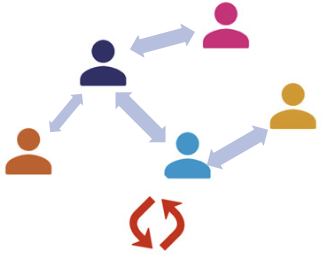
\includegraphics[width=3.38cm]{figures_zh/ch17/abm_people}};
  \node[inner sep=0pt] at (1.92,1.95)
    {
\includegraphics[width=3.28cm]{figures_zh/ch17/abm_environments}};
  \node[font=\fontsize{8}{10}\selectfont] at (.56,1.36) {物理};
  \node[font=\fontsize{8}{10}\selectfont] at (1.48,1.36) {社会};
  \node[font=\fontsize{8}{10}\selectfont] at (2.35,1.36) {网络};
  \node[font=\fontsize{8}{10}\selectfont] at (3.23,1.36) {混合};
  \node[req] (abm-social) at (5.38,5.55) {社会能力};
  \node[req] (abm-autonomy) at (5.38,4.22) {自主性};
  \node[req] (abm-reactivity) at (5.38,2.89) {反应性};
  \node[req] (abm-proactive) at (5.38,1.56) {主动性};
  \node[ability] (abm-perception) at (8.92,5.55) {感知};
  \node[ability] (abm-reason) at (8.92,4.22) {推理};
  \node[ability] (abm-decision) at (8.92,2.89) {决策};
  \node[ability] (abm-evolution) at (8.92,1.56) {自我演化};
  \foreach \from/\to in {perception/social,reason/social,
    reason/reactivity,decision/autonomy,decision/proactive,
    evolution/proactive}
    \draw[dashed,->] (abm-\from.west) -- (abm-\to.east);
  \draw[dashed,<->] (abm-reason.west) -- (abm-autonomy.east);
  \draw[dashed,<->] (abm-decision.west) -- (abm-reactivity.east);
  \draw[decorate,decoration={brace,amplitude=6pt}] (4.10,1.43) -- (4.10,5.53);
  \draw[decorate,decoration={brace,amplitude=6pt}] (10.38,5.58) -- (10.38,1.43);
  \draw[densely dotted,thick] (10.77,1.02) rectangle (15.52,5.98);
  \node[inner sep=0pt] at (11.60,3.60)
    {
\includegraphics[width=1.45cm]{figures_zh/ch17/abm_robot}};
  \node[font=\fontsize{7}{9}\selectfont] at (11.60,2.48) {大语言模型};
  \foreach \name/\y/\txt in {interface/5.12/接口,mechanism/3.58/内部机制,action/2.02/动作}
    \node[draw=blue!40!black,fill=orange!70!brown,text=white,ellipse,
      minimum width=2.50cm,minimum height=.72cm,font=\small] (abm-\name) at (14.03,\y) {\txt};
  \draw[->,orange!80!black,line width=1.5pt] (abm-interface.south) -- (abm-mechanism.north);
  \draw[->,orange!80!black,line width=1.5pt] (abm-mechanism.south) -- (abm-action.north);
  \node[font=\small\bfseries,align=center] at (3.48,.40) {基于智能体的建模\\与模拟的要求};
  \node[font=\small\bfseries,align=center] at (11.04,.40) {大语言模型\\智能体的能力};
\end{tikzpicture}
